   \subsection{Beam Energy}
 
   30GeV proton beam hits to target T1 in Hadron hall.
   It generates many particles like kaon, pion, muon, electron, and
   so on.
   We take the particles that has 800MeV/c momentum from this beam by
   using D1 magnet.\\
   \ \ For this analysis, a beam momentum at BDC after passing through the
   K1.1Br beam line is required.
   We estimate a beam momentum using simple MC simulation.
   Figure \ref{K11Br_Beam_line} shows MC simulation's geometory.
   This time, beam line is straight and has no electric and magnetic
   field.
   MC simulation shoot 800MeV/c kaon and pion as pencil beam.

   Figure \ref{k_pi_momentum} shows kaon and pion momentum distribution
   using this MC simulation.
   Actually, kaon momentum distribution peak is adjusted so that kaon
   decay point of MC simulation is consistent with data.
   Section \ref{kaon_energy_section} explains this point.
   And proton momentum is estimated in other way, using TREK detector
   TOF information.
   Section \ref{proton_energy_section} shows proton momentum distribution.

   \subsubsection{Kaon energy}\label{kaon_energy_section}

We adjust momentum peak of figure ?? and set Kaon beam energy  the point that the decay points of Kaon in data and simulation are good agreement. The distribution of decay poins are plotted in Figure\ref{DecayPoint_hough}.
\begin{figure}[!htb]
  \begin{center}
    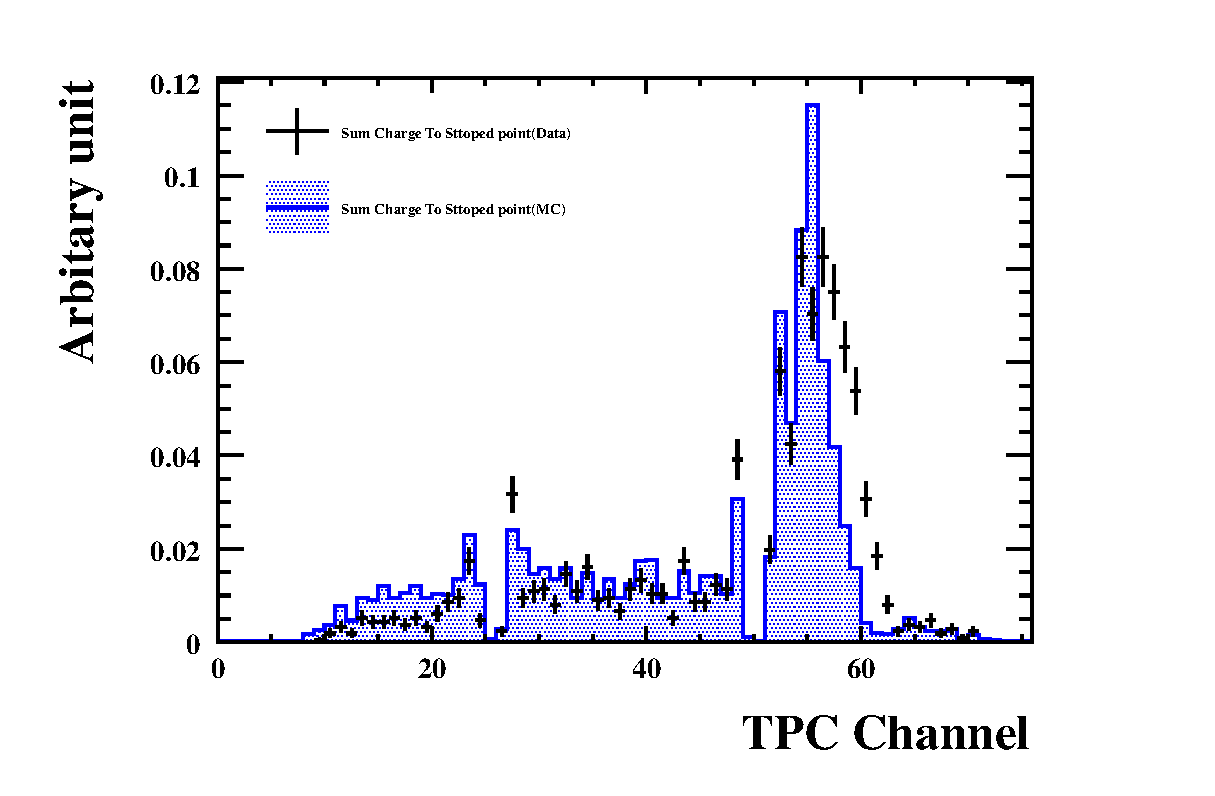
\includegraphics[width=70mm]{fig/cdp_hough.eps}
  \end{center}
  \caption{Decay point distribution of Data and MC}
  \label{DecayPoint_hough}
\end{figure}

   \subsubsection{Proton energy}\label{proton_energy_section}

Beam momentum is ideally TOF information,
but considered the dispersion, we should take into account of the resolution of TOF.
As we know the resolution of TOF is $\sim$200ps beforehand,
we can calculate the effect of this resolution to beam momentum.
For example, as shows in table\ref{tb:TOF_expect}, 
the time of flight of 800MeV/c $K^{+}$ between two TOF Counters is 13.71$ns$.
When considering 0.2$ns$ TOF resolution for this value,
the momentum is approximately 760$\sim$845MeV/c spreading largely.
However, taking the same calculation for 800MeV/c $p$,
the momentum is approximately 785$\sim$815MeV/c surpressing the dispersion to some extent.
In addition, because the dispersion of Time of Flight of $p$ appears widespread over TOF resolution,
we estimate the momentum of $p$ from TOF information.\\
Figure\ref{fig:Proton_tof} shows responce of TOF Counters of PhysicsOct49 whose data include many $p$ events.
As discribed above, the holizontal axis don't show the real time of flight.
Then, with PhysicsOct47 whose data include much $e^{+}$ events, we determined the mean of $e^{+}$.
As the $beta$ of $e^{+}$ is $\sim$1.0, this value of horizontal axis correspond 11.67$ns$(dotted line in Fig\ref{fig:Proton_tof}).
Figure\ref{fig:Proton_momentum} shows the estimated momentum histgram from figure\ref{fig:Proton_tof}
and this momentum distribution is implemented to Monte Carlo Simulation.
Whether the distribution reproduce DATA well is discussed in section 7.2.

\begin{figure}[htbp]
  \begin{tabular}{cc}
    \begin{minipage}{0.5\hsize}
      \centering
      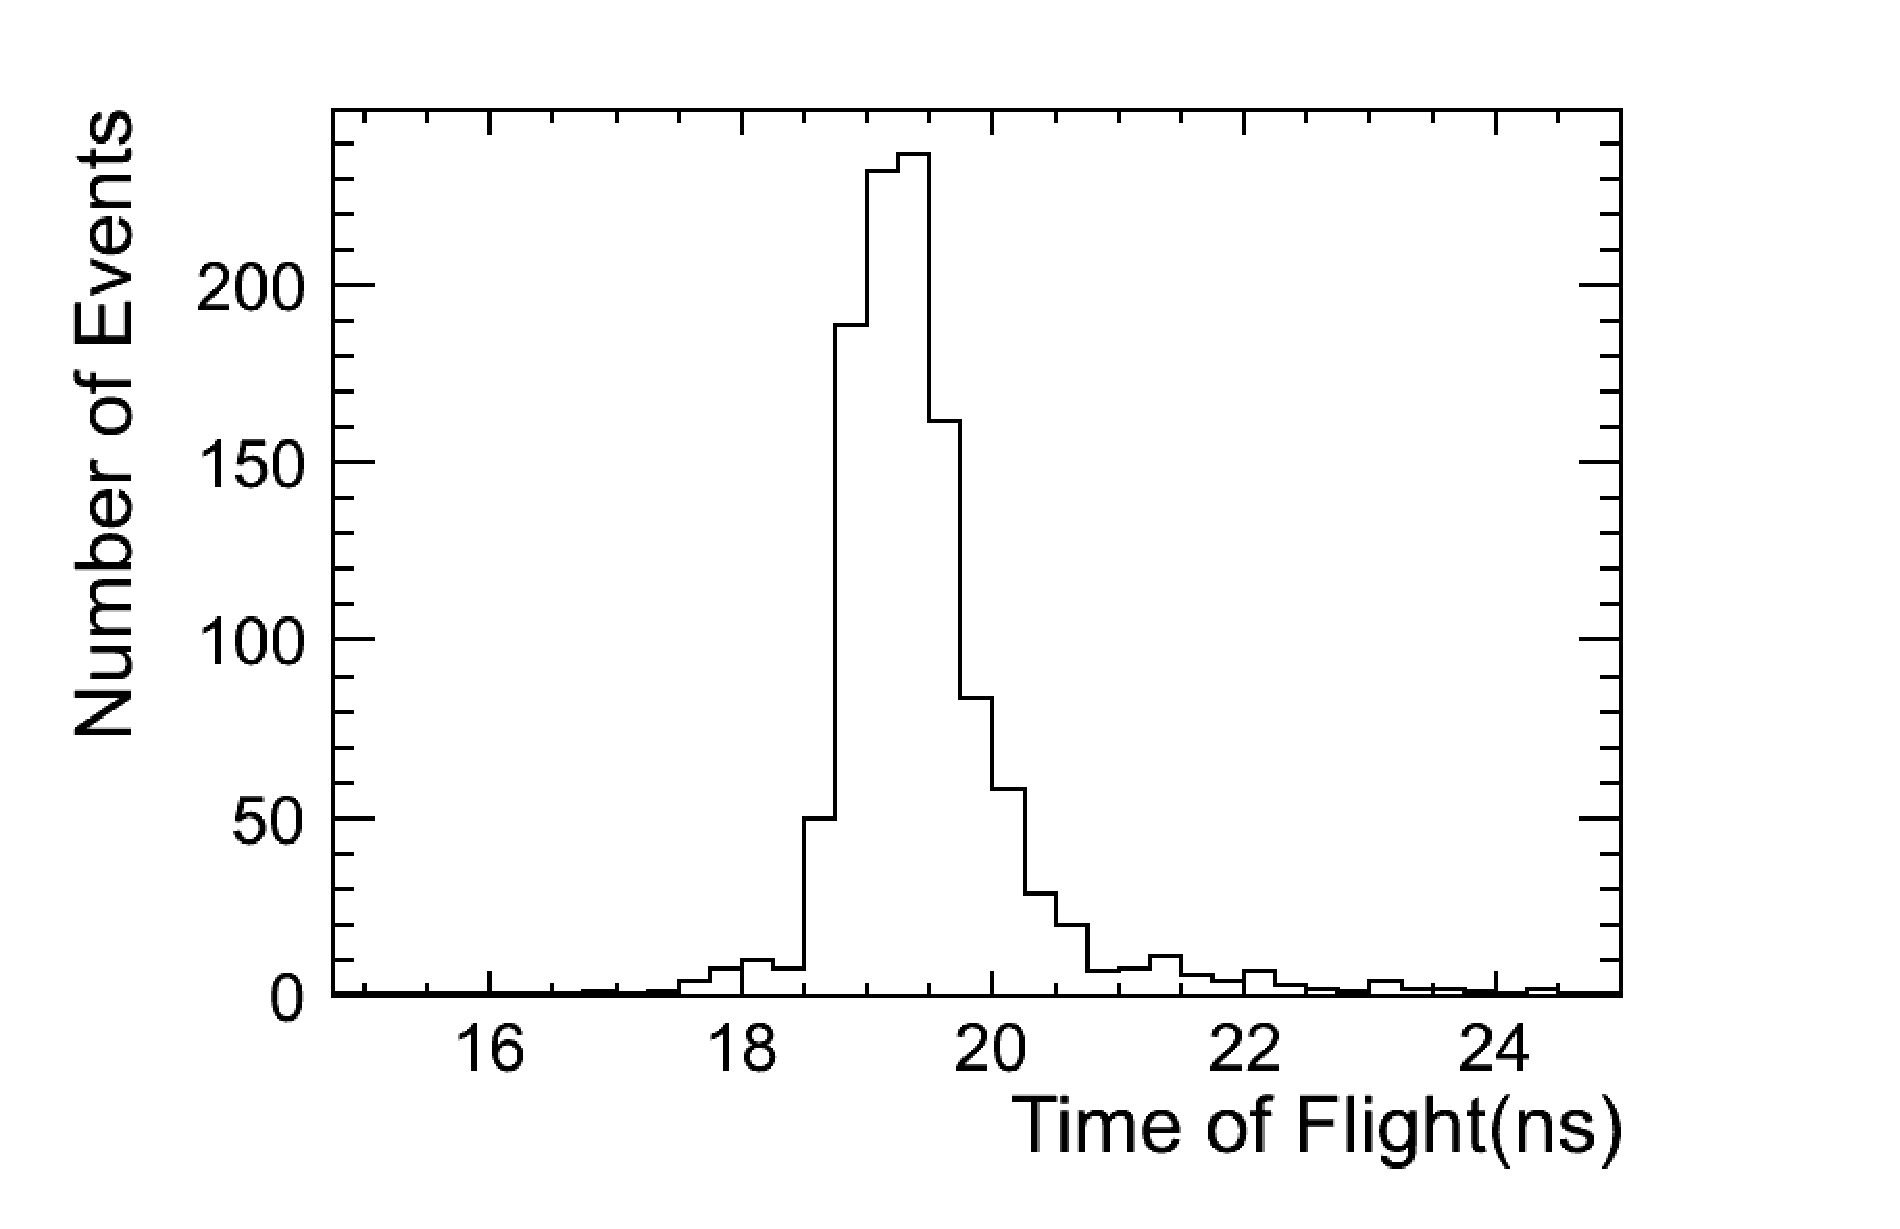
\includegraphics[width=6cm,clip]{fig/TOF_proton.eps}
      \caption{$p$ TOF response}
      \label{fig:Proton_tof}
    \end{minipage}
    \begin{minipage}{0.5\hsize}
      \centering
      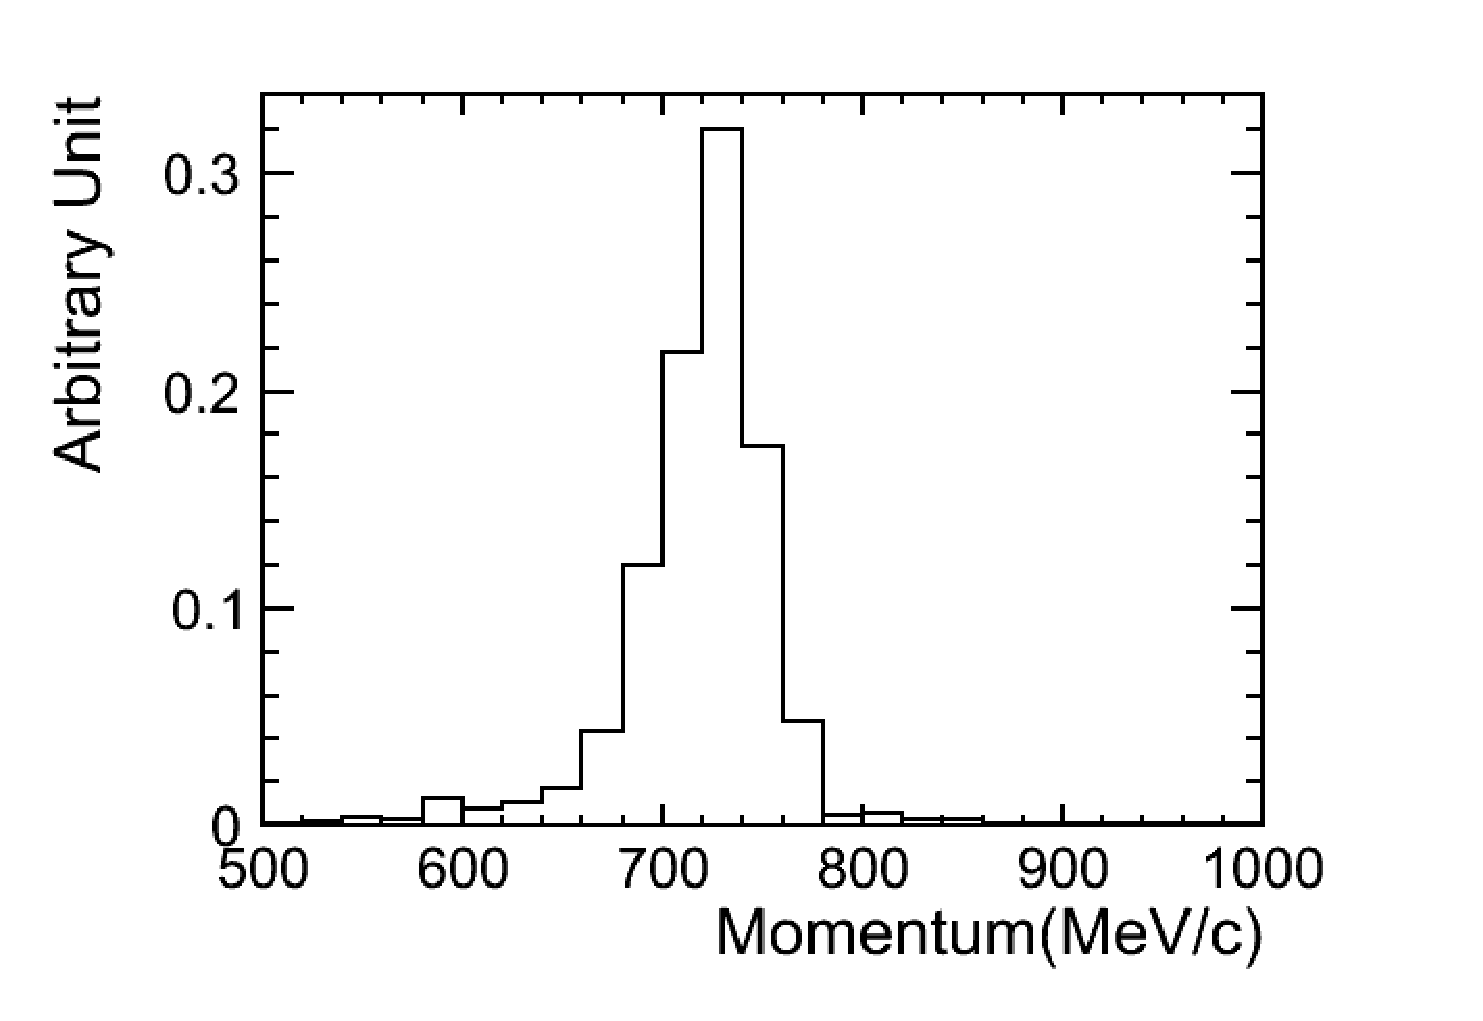
\includegraphics[width=6cm,clip]{fig/Momentum_proton.eps}
      \caption{Estimated $p$ momentum}
      \label{fig:Proton_momentum}
    \end{minipage}
  \end{tabular}
\end{figure} 

   \subsubsection{Energy deposition in degrader}
   Because of having high energy, kaon beam from BDC passes through 250LAr TPC.
   So that kaon stops in 250LAr TPC, we put degrader, which reduce
   beam energy, on beam line.
   In this experiment, we used lead glass and lead block as degrader.
   We estimate energy deposition in degrader by using MC simulation.
   Figure \ref{energy_deposition} shows energy deposition in degrader.
   
   \subsection{Beam Position}
   Before taking data, we measured a beam profile on the front of
   250LAr TPC by using plastic scintillation counter.
   Figure \ref{beamprofile_250L} shows beam profile on the front of
   250LAr TPC.

   \begin{figure}[!htb]
    \centering
    \centering
    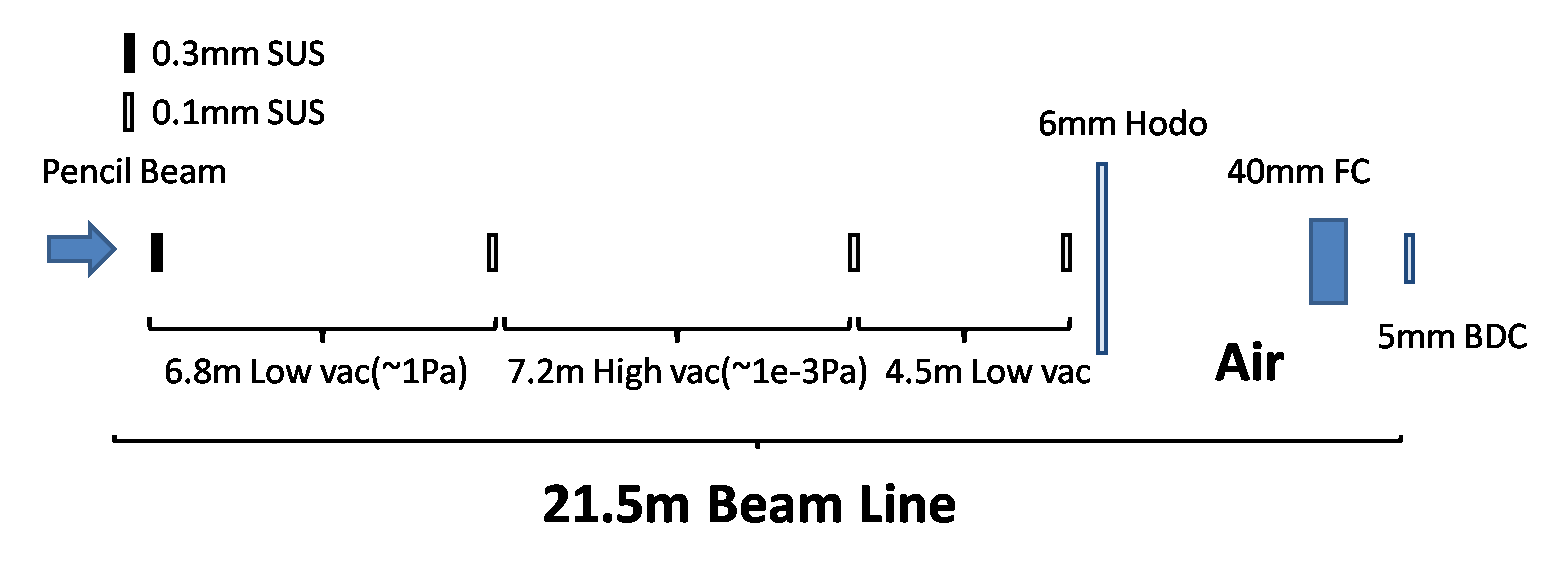
\includegraphics[width=11cm,clip]{./fig/K11Br_beamline_sim.eps}
    \caption{K1.1 Br beamline}
    \label{K11Br_Beam_line}
   \end{figure}



   \begin{figure}[!htb]
    \centering
    \centering
    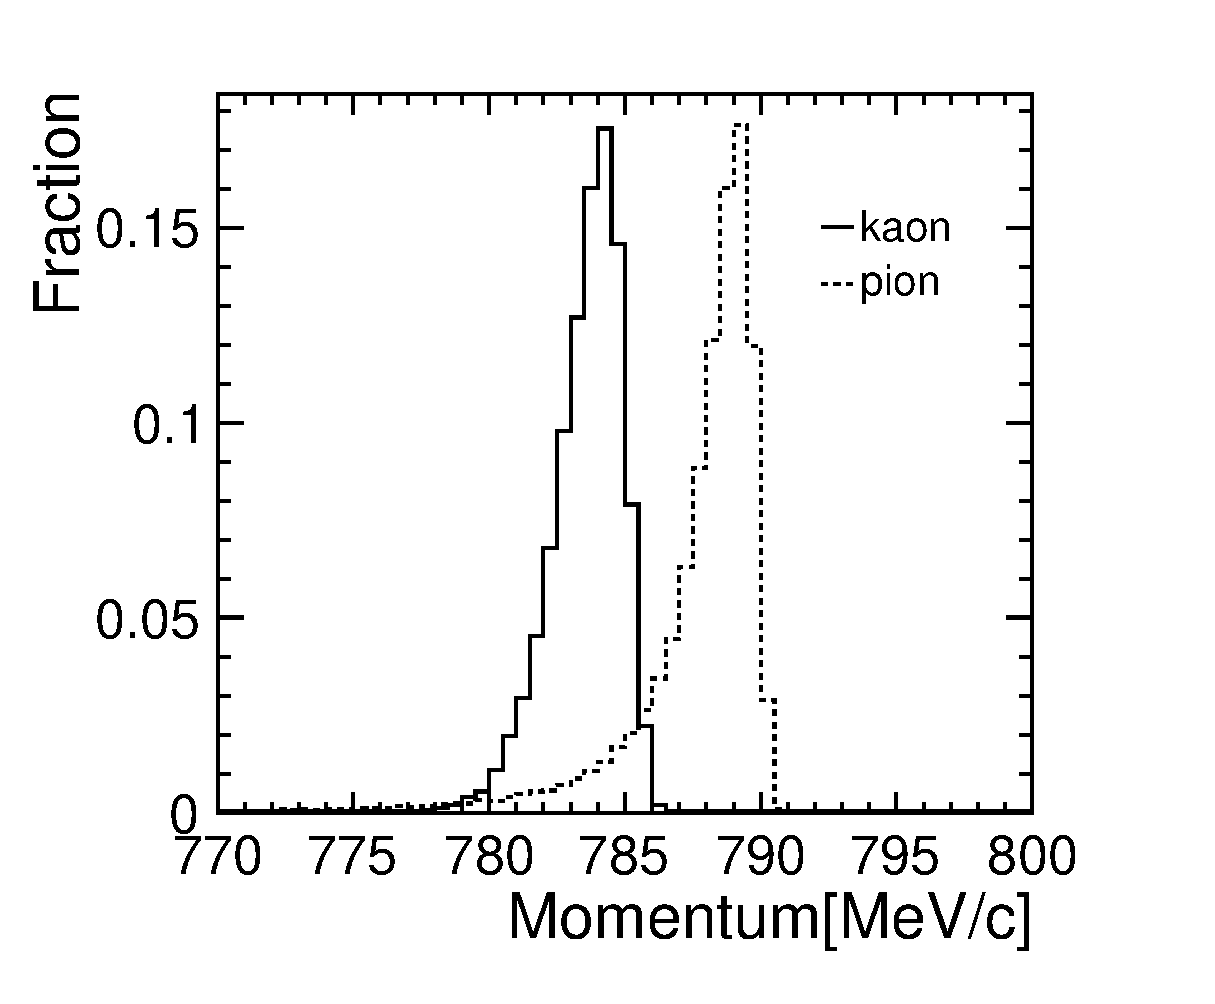
\includegraphics[width=11cm,clip]{./fig/Kaon_pion_momentum_nogrid.eps}
    \caption{kaon and pion momentum distribution at BDC}
    \label{k_pi_momentum}
   \end{figure}


   \begin{figure}[!htb]
    \centering
    \centering
    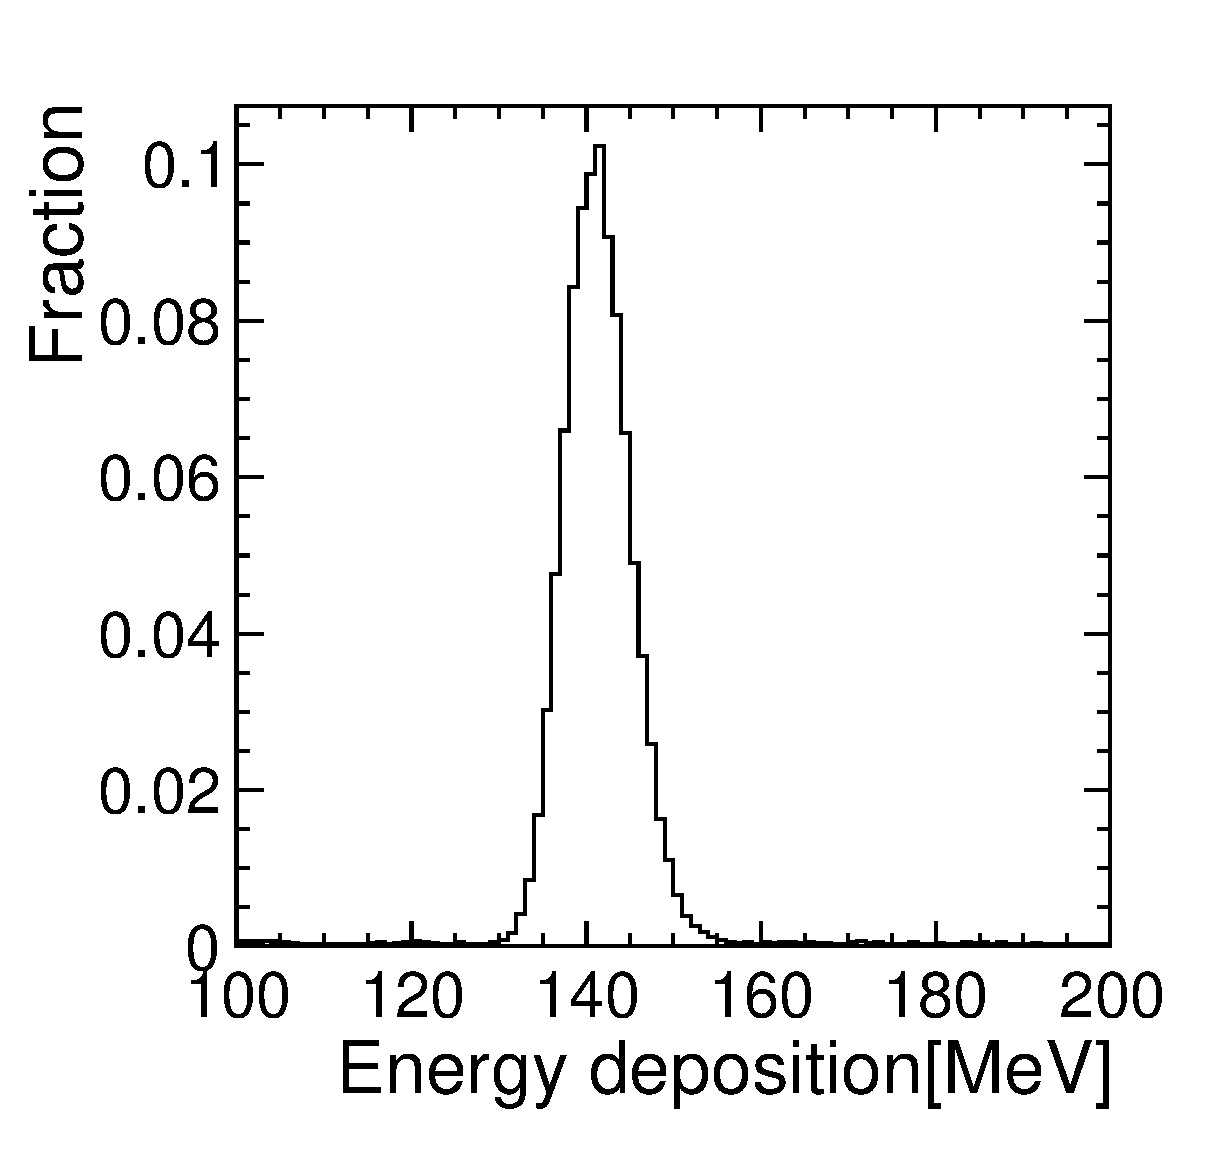
\includegraphics[width=11cm,clip]{./fig/energy_deposition.eps}
    \caption{energy deposition in degrader}
    \label{energy_deposition}
   \end{figure}


   \begin{figure}[!htb]
    \centering
    \centering
    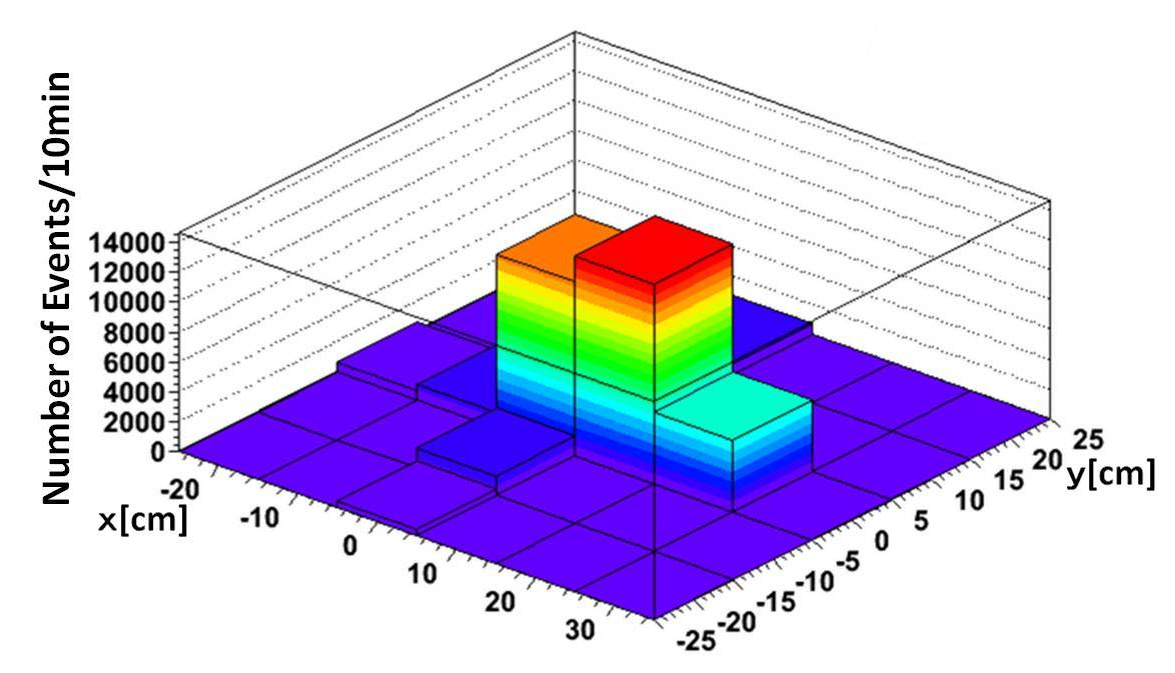
\includegraphics[width=11cm,clip]{./fig/BeamProfile3.eps}
    \caption{Beam profile on the front of 250LAr TPC}
    \label{beamprofile_250L}
   \end{figure}
